\begin{table}[!h]
\centering
\caption{Monte Carlo Design Parameters}
\label{tab:mc_design}
\begin{tabular}{ccccc}
\toprule
Sample Size $n$ & Subsample Size $b$ & Non-overlapping Blocks $N_b$ & MC Replications $M$ \\
\midrule
500{,}000 & 6{,}299 & 79 & 200 \\
\bottomrule
\end{tabular}
\begin{flushleft}
\footnotesize\textit{Notes:} The subsample size is set to $b = \lfloor n^{2/3} \rfloor$ following \cite{PR99}.  $N_b = \lfloor n/b \rfloor$ denotes the number of non-overlapping blocks per replication.
\end{flushleft}
\end{table}


\begin{table}[!h]
\centering
\caption{Summary of unrestricted subsampling results (reparameterized space)}
\label{tab:subsampling_summary}
\resizebox{\textwidth}{!}{%
\begin{tabular}{lccccccccccc}
\toprule
& & & & & & & \multicolumn{2}{c}{Quantile CI} & \multicolumn{2}{c}{Normal CI} \\
\cmidrule(lr){8-9} \cmidrule(lr){10-11}
$n$ & Param.\ & True & Avg.\ Est.\ & Std.\ Est.\ & Dev.\ Mean & Skew & Kurt & qCov90 & qCov95 & nCov90 & nCov95 \\
\midrule
\multirow{5}{*}{$500{,}000$}
& $\psi_1$ & 0.80 & 0.800 & 0.003 & $0.03$ & $0.49$ & $1.53$ & 0.925 & 0.965 & 0.910 & 0.950 \\
& $\psi_2$ & 0.30 & 0.299 & 0.006 & $-0.30$ & $-0.73$ & $1.63$ & 0.940 & 0.965 & 0.955 & 0.980 \\
& $\sigma$ & 1.60 & 1.599 & 0.006 & $-0.35$ & $-0.06$ & $0.14$ & 0.940 & 0.960 & 0.930 & 0.955 \\
& $\pi_1$ & 0.4375 & 0.437 & 0.005 & $0.01$ & $-0.33$ & $1.44$ & 0.925 & 0.970 & 0.930 & 0.965 \\
& $\alpha$ & 1.50 & 1.500 & 0.004 & $0.04$ & $0.01$ & $-0.01$ & 0.910 & 0.950 & 0.900 & 0.945 \\
\bottomrule
\end{tabular}%
}
\begin{flushleft}
\footnotesize\textit{Notes:} Avg.~Est.\ and Std.~Est.\ are the mean and standard deviation of $\hat{\vartheta}_n$ over $M=200$ replications.  Dev.~Mean, Skew, and Kurt are the mean, skewness and excess kurtosis of the non-overlapping block scaled deviations $Z^{(i)}_b$, pooled across replications.  qCov and nCov denote the average coverage of quantile-based and normal-approximation confidence intervals.  The full-sample and block estimators are the same functional, evaluated with identical starting values and optimizer tolerances.
\end{flushleft}
\end{table}


\begin{table}[htbp]
\centering
\caption{Subsampling results (reparameterized) for $n = 500{,}000$ ($b = 6{,}299$, $N_b = 79$, $M = 200$)}
\label{tab:subsampling_n500000}
\resizebox{\textwidth}{!}{%
\begin{tabular}{lcccccccccccccc}
\toprule
& & & & & & & & & \multicolumn{2}{c}{Quantile CI} & \multicolumn{2}{c}{Normal CI} \\
\cmidrule(lr){10-11} \cmidrule(lr){12-13}
Parameter & True & Avg Est.\ & Std Est.\ & Dev.\ Mean & Dev.\ Std & Skew & Kurt & SW Rej.\ & JB Rej.\ & qCov90 & qCov95 & nCov90 & nCov95 \\
\midrule
$\rho_1$ & 0.800 & 0.800 & 0.003 & $0.03$ & 2.099 & $0.49$ & $1.53$ & 0.260 & 0.275 & 0.925 & 0.965 & 0.910 & 0.950 \\
$\rho_2$ & 0.300 & 0.299 & 0.006 & $-0.30$ & 4.779 & $-0.73$ & $1.63$ & 0.460 & 0.420 & 0.940 & 0.965 & 0.955 & 0.980 \\
$\sigma$ & 1.600 & 1.599 & 0.006 & $-0.35$ & 5.045 & $-0.06$ & $0.14$ & 0.090 & 0.065 & 0.940 & 0.960 & 0.930 & 0.955 \\
$\pi_1$ & 0.437 & 0.437 & 0.005 & $0.01$ & 4.251 & $-0.33$ & $1.44$ & 0.170 & 0.195 & 0.925 & 0.970 & 0.930 & 0.965 \\
$\alpha$ & 1.500 & 1.500 & 0.004 & $0.04$ & 2.763 & $0.01$ & $-0.01$ & 0.070 & 0.045 & 0.910 & 0.950 & 0.900 & 0.945 \\
\bottomrule
\end{tabular}%
}
\begin{flushleft}
\footnotesize\textit{Notes:} All results are in the reparameterized space $(\rho_1, \rho_2, \sigma, \pi_1, \alpha)$.  The full-sample estimator $\hat{\vartheta}_n$ and every block estimator $\hat{\vartheta}^{(i)}_b$ are the same functional: identical criterion, grid, starting values, bounds and optimizer tolerances, as required by the subsampling theory of \cite{PR94}.  Dev.~Mean, Dev.~Std, Skew and Kurt are computed on the non-overlapping block deviations $Z^{(i)}_b$ pooled across all $M = 200$ replications (15{,}800 values per parameter).  SW and JB rejection rates are per-replication rejection frequencies at the 5\% level.  qCov and nCov denote quantile-based and normal-approximation CI coverage; confidence intervals use the 1{,}999 overlapping blocks (thinned with step 247 out of $n - b + 1 = 493{,}702$), while the normality diagnostics use the non-overlapping blocks.
\end{flushleft}
\end{table}


\begin{figure}[htbp]
\centering
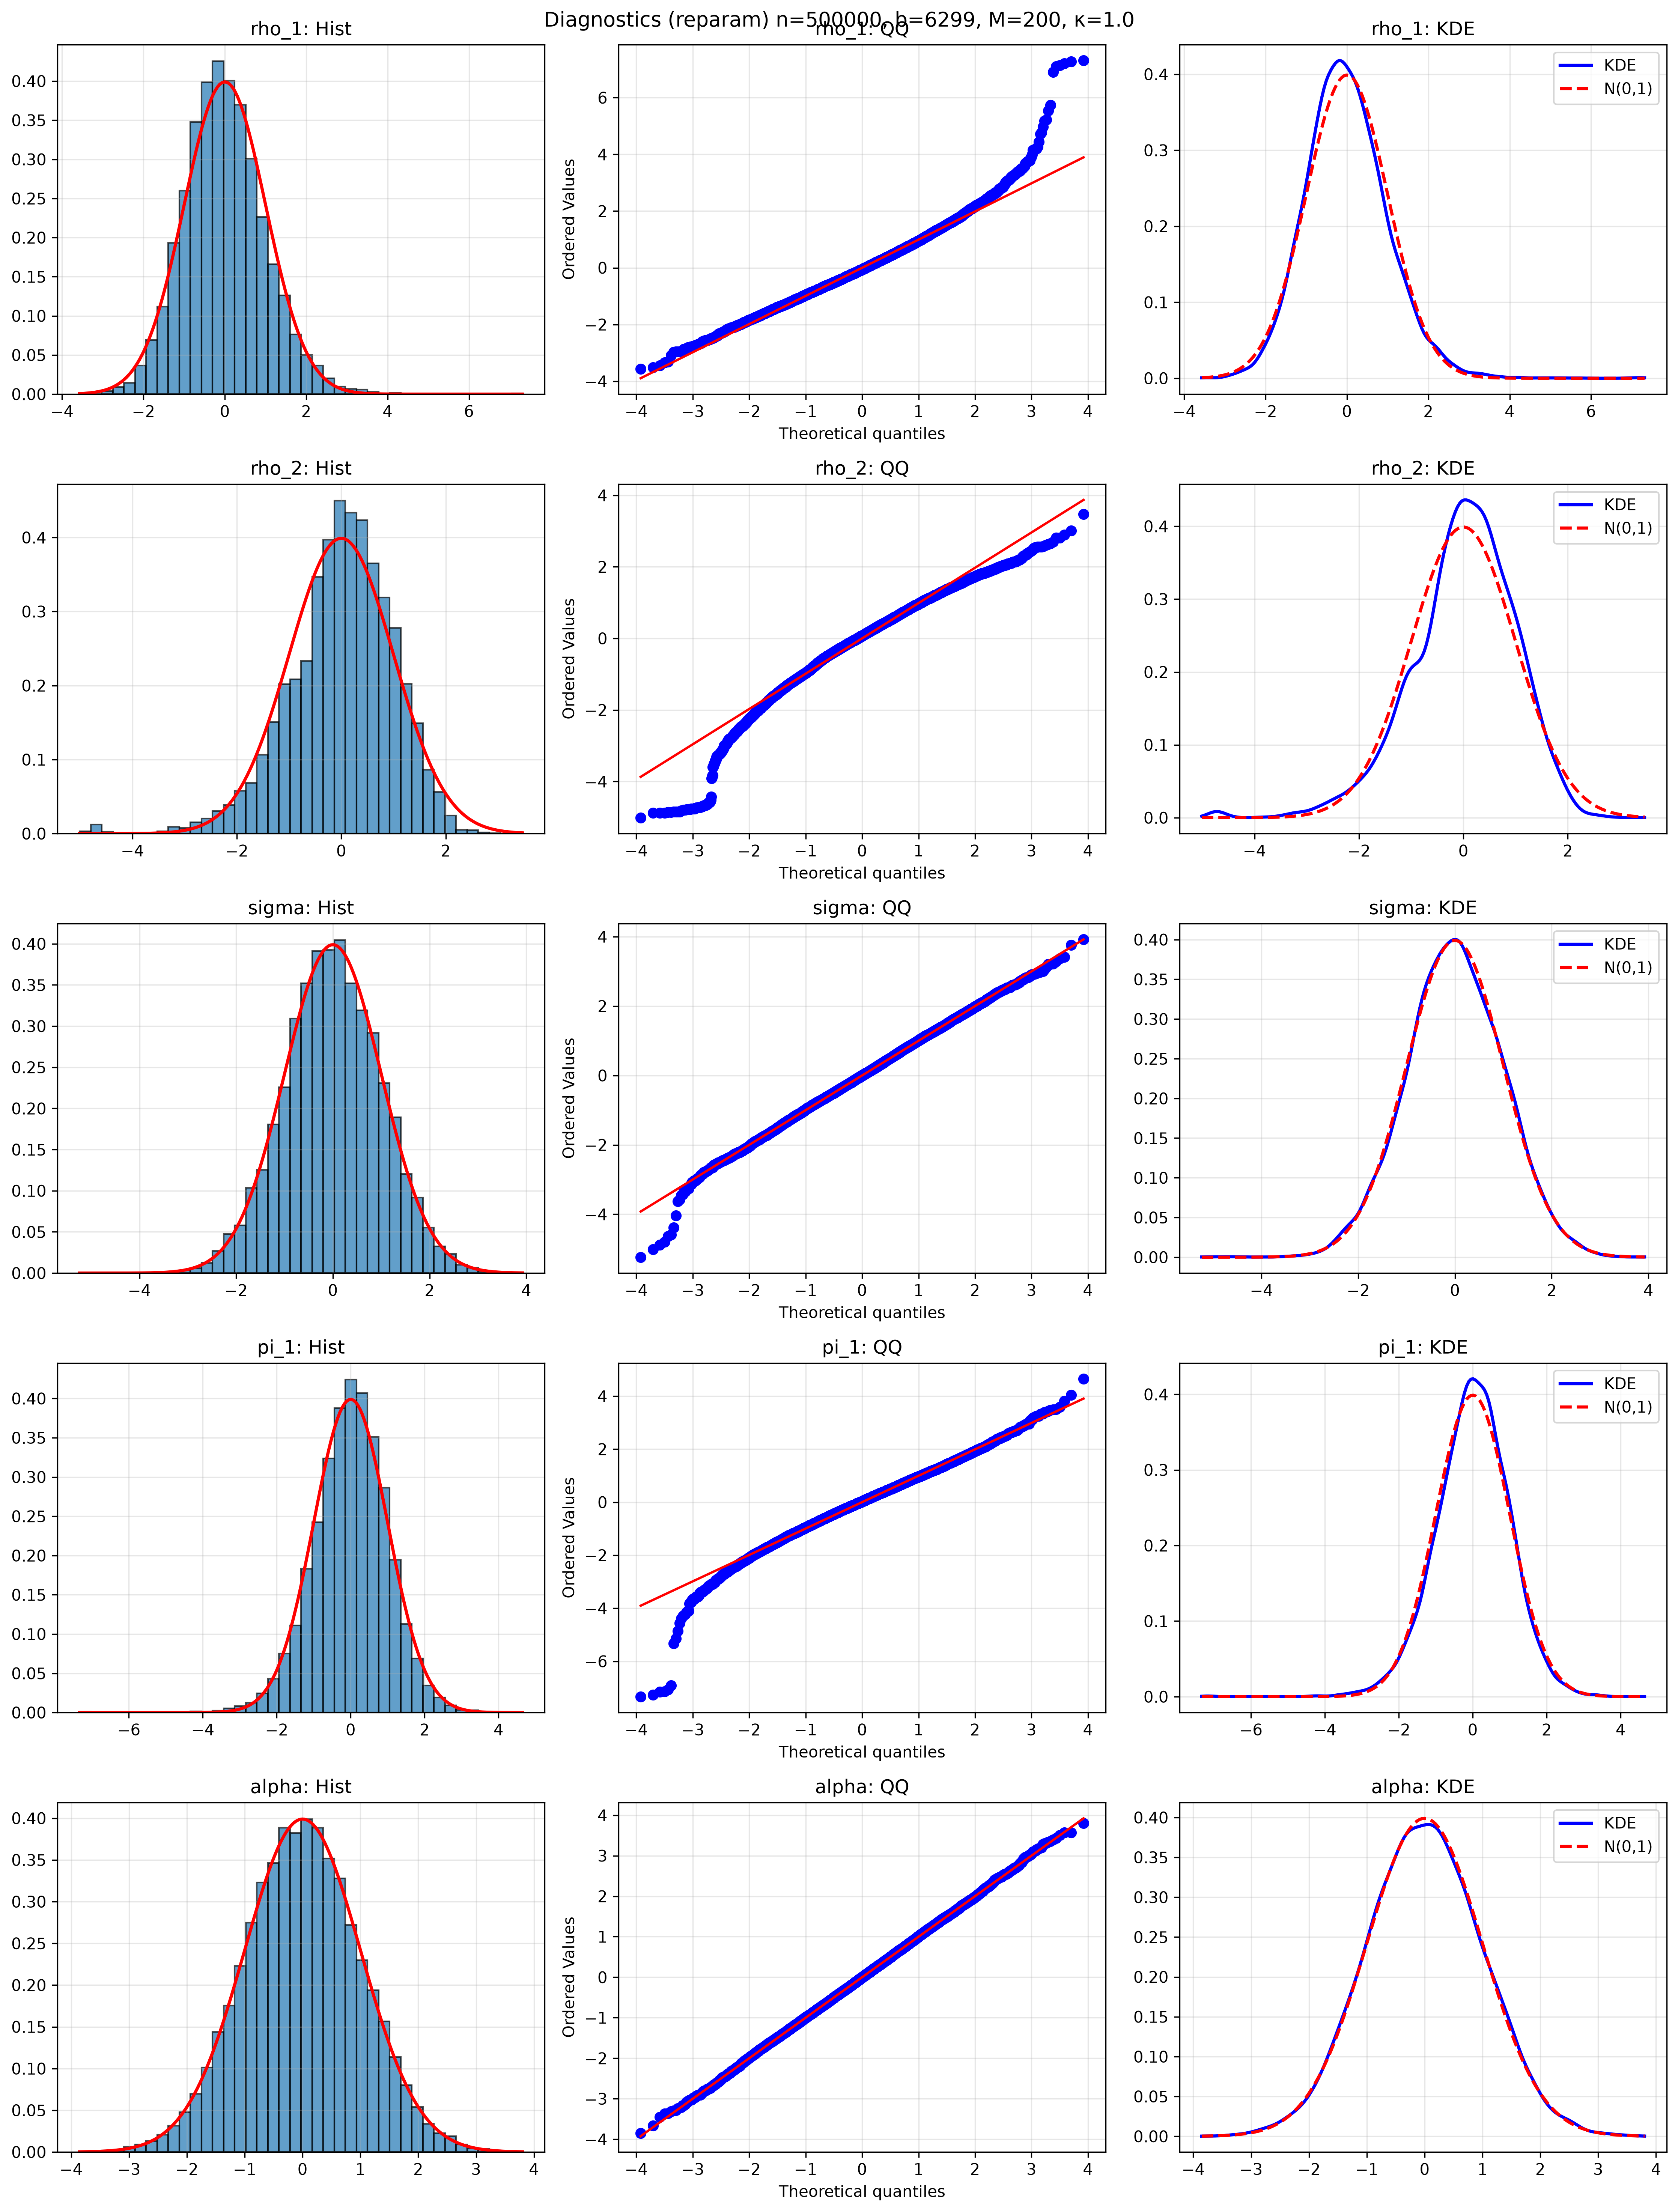
\includegraphics[width=\textwidth]{resultats_reparam/diagnostics_n500000.png}
\caption{Diagnostic plots for scaled subsample deviations (reparameterized) at $n = 500{,}000$. For each parameter (rows), we display: (left) histogram with standard normal overlay, (center) Q-Q plot against standard normal quantiles, and (right) kernel density estimate compared to the standard normal density.}
\label{fig:diagnostics_n500000}
\end{figure}
